\chapter{Estado del Arte}

\section{Librerías de visualización de estructuras de datos}

Actualmente existen varias librerías para generar visualizaciones de estructuras de datos, pero muchas de ellas están implementadas en lenguajes distintos de Python y no están diseñadas para poder ser utilizadas en Notebooks.
Un ejemplo de esto es la librería Reftree~\cite{Stanch2021} que permite crear visualizaciones de estructuras de datos, pero en el lenguaje Scala, por lo tanto, no se puede utilizar para visualizar estructuras de datos implementadas en Python y tampoco se puede utilizar en Jupyter Notebooks.
Otro ejemplo es la librería Lolviz~\cite{Lolviz} que, si bien si permite visualizar en Notebooks estructuras de datos implementadas en Python, cuenta con la limitación de que no puede generar animaciones. En la figura \ref{fig:comparacion} se pueden ver ejemplos de las visualizaciones generadas por estas librerías.

\begin{figure}[h!]%
    \centering
    \subfloat[Reftree]{
        \centering
        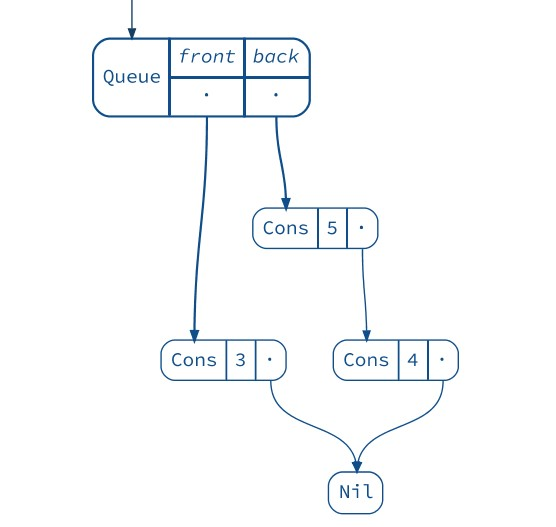
\includegraphics[width=\dimexpr(\linewidth-12pt)/2\relax, height=\dimexpr(\linewidth-12pt)/2\relax]{imagenes/ejemplos/reftree}
        \label{fig:reftree}
    }
    \subfloat[Lolviz]{
        \centering
        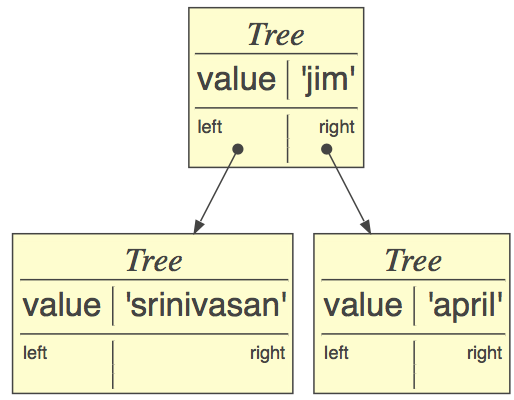
\includegraphics[width=\dimexpr(\linewidth-12pt)/2\relax]{imagenes/ejemplos/lolviz}
        % \vspace{38px}
        \label{fig:lolviz}
    }\\
    \subfloat[Aed Utilities]{
        \centering
        \includesvg[width=\dimexpr(\linewidth-12pt)/2\relax]{imagenes/ejemplos/aed}
        \label{fig:aed}
    }
    \subfloat[Manim]{
        \centering
        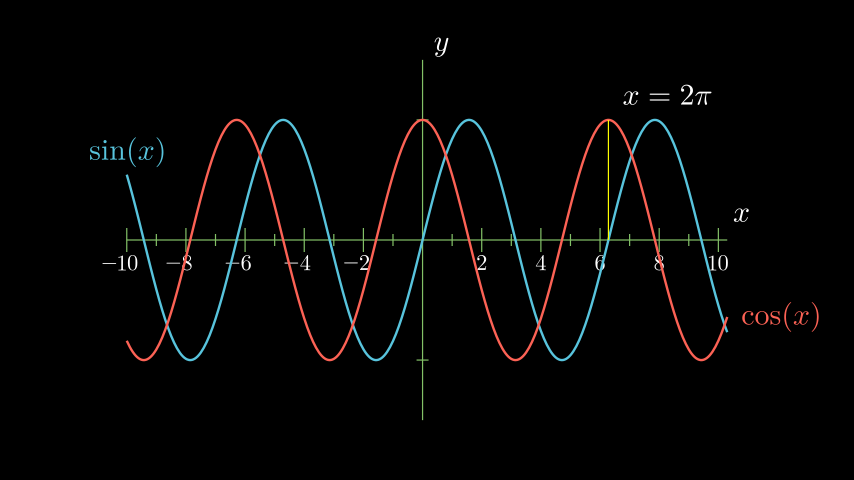
\includegraphics[width=\dimexpr(\linewidth-12pt)/2\relax]{imagenes/ejemplos/manim}
        \label{fig:manim}
    }
    \caption[Ejemplos de las distintas herramientas.]{Ejemplos de visualizaciones generadas por las distintas herramientas. Obtenidas de \cite{Stanch2021}, \cite{Lolviz}, \cite{aed-utilities} y \cite{manim}, respectivamente.}
    \label{fig:comparacion}
\end{figure}

Por otro lado, existe la librería Aed-Utilities~\cite{aed-utilities} creada para el curso de Algoritmos y Estructuras de Datos de la FCFM por el Profesor Ivan Sipiran; que, si bien permite generar diagramas de estructuras de datos en Python y mostrarlas en un Notebook, cuenta con las siguientes limitaciones: no permite crear animaciones, la API no es muy cómoda de utilizar y el algoritmo que utiliza para generar las visualizaciones es poco eficiente. % TODO: Explicar

Tanto Aed-Utilites como Lolviz generan los diagramas utilizando Graphviz ---una herramienta originalmente desarrollada por AT\&T para dibujar gráficos especificados en el lenguaje DOT--- que permite generar diagramas de muy buena calidad, pero no permite crear animaciones.

En cuanto a las herramientas para generar animaciones, existe la librería Manim~\cite{manim}, diseñada para generar visualizaciones animadas de matemáticas. Si bien no está diseñada para crear visualizaciones de estructuras de datos, es relevante porque permite generar animaciones y estas animaciones se pueden ver desde Notebooks. Esta librería tiene un diseño orientado a objetos, donde una animación es un objeto que tiene un campo con el objeto matemático que representa y tiene un método que permite animar el objeto según una función de interpolación. Para generar el resultado final puede utilizar varios back-ends de rendering, incluyendo OpenGL y WebGL. Utilizando este último cuando se usa desde un Notebook. En la figura \ref{fig:manim} se puede ver una visualización de una función creada con esta herramienta.

Otra herramienta enfocada en las matemáticas es Penrose~\cite{Penrose}, una herramienta que permite crear diagramas a partir de un programa en un lenguaje específico de dominio. La disposición de los elementos en el diagrama se obtiene mediante optimización numérica. El lenguaje específico de dominio (o DSL por sus iniciales en inglés) se separa en un archivo que define solo la parte matemática y en otro que define el estilo.

Dado que no se encontró ninguna herramienta existente que permita visualizar estructuras de datos implementadas en Python, permita generar animaciones y permita mostrar las visualizaciones generadas en un Jupyter Notebooks, se requiere crear una nueva librería que implemente esta funcionalidad.

\section{Jupyter Notebooks}

Los Jupyter Notebooks son archivos interactivos que almacenan bloques de texto, código y también pueden contener imágenes, videos y animaciones interactivas. Un Jupyter Notebook tiene varios componentes que permiten construir la experiencia de usuario. En primer lugar, está el archivo del notebook que es un archivo JSON con la extensión \texttt{.ipynb}, que almacena en el disco todos los datos persistentes del notebook, incluyendo los bloques de texto, los bloques de código y sus salidas, las imágenes, etc. Después, está el \textit{kernel} o núcleo, que es un intérprete del lenguaje respectivo, con la capacidad de comunicarse con el servidor del notebook. El servidor del notebook se encarga de la comunicación entre el front-end, el kernel y el archivo del notebook. Finalmente, está el front-end del notebook, que se encarga de mostrarle al usuario una representación del notebook y le permite a este interactuar con el notebook, usualmente corresponde a un navegador web. En la figura \ref{fig:notebook_arq} se puede ver un diagrama de esta arquitectura.

\begin{figure}[h]
  \centering
  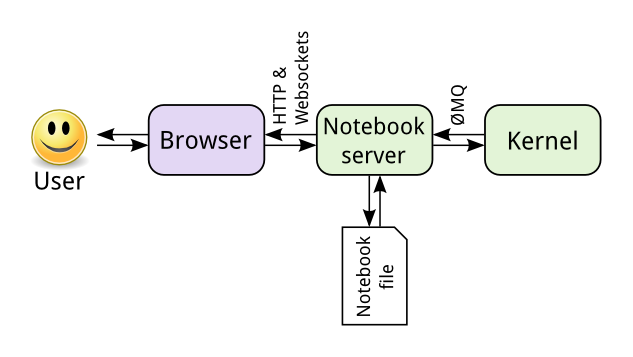
\includegraphics[width=\textwidth]{imagenes/notebook/notebook_components}
  \caption[Arquitectura de Jupyter Notebooks]{Arquitectura de Jupyter Notebooks. Obtenido de \cite{arq-notebook}.}
  \label{fig:notebook_arq}
\end{figure}

\begin{figure}[h]
    \centering
    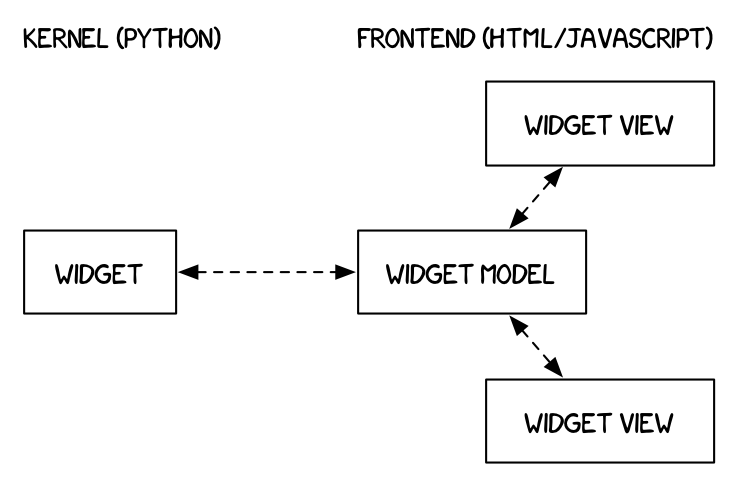
\includegraphics[width=0.8\textwidth]{imagenes/notebook/WidgetModelView}
    \caption[Arquitectura de Jupyter Widgets]{Arquitectura de Jupyter Widgets. Obtenido de \cite{arq-widget}.}
    \label{fig:widget_arq}
\end{figure}

Existen múltiples kernels, uno por cada lenguaje que soportan los Jupyter Notebooks, pero el más conocido es el kernel IPython que es el kernel del lenguaje Python. IPython además de ser un kernel de Jupyter Notebooks es un intérprete interactivo de Python, con funcionalidades como contenido multimedia y completado de comandos. Cuando se utiliza un notebook con el lenguaje Python, el servidor del notebook se comunica con este intérprete que es que se encarga de interpretar los bloques de código y responder con la salida generada cuando el servidor del notebook envía el request.

Para crear componentes interactivos en un Notebook de Python se utiliza la librería Jupyter Widgets. Esta librería permite definir un modelo que representa el componente, y una vista en JavaScript y HTML que es mostrada por el front-end del Notebook. El modelo se define tanto en JavaScript como en Python y la librería se encarga de mantener las dos versiones sincronizadas. Para mantener las dos versiones sincronizadas, es necesario serializar y deserializar los campos del modelo, para poder enviarlos en formato JSON. Entonces, para los campos sencillos, la librería se puede encargar de la serialización o deserialización, pero para los casos más complejos se deben definir manualmente los serializadores y deserializadores para cada campo. En la figura \ref{fig:widget_arq} se observa la arquitectura de un widget generado con esta librería.

\begin{figure}[H]
    \centering
    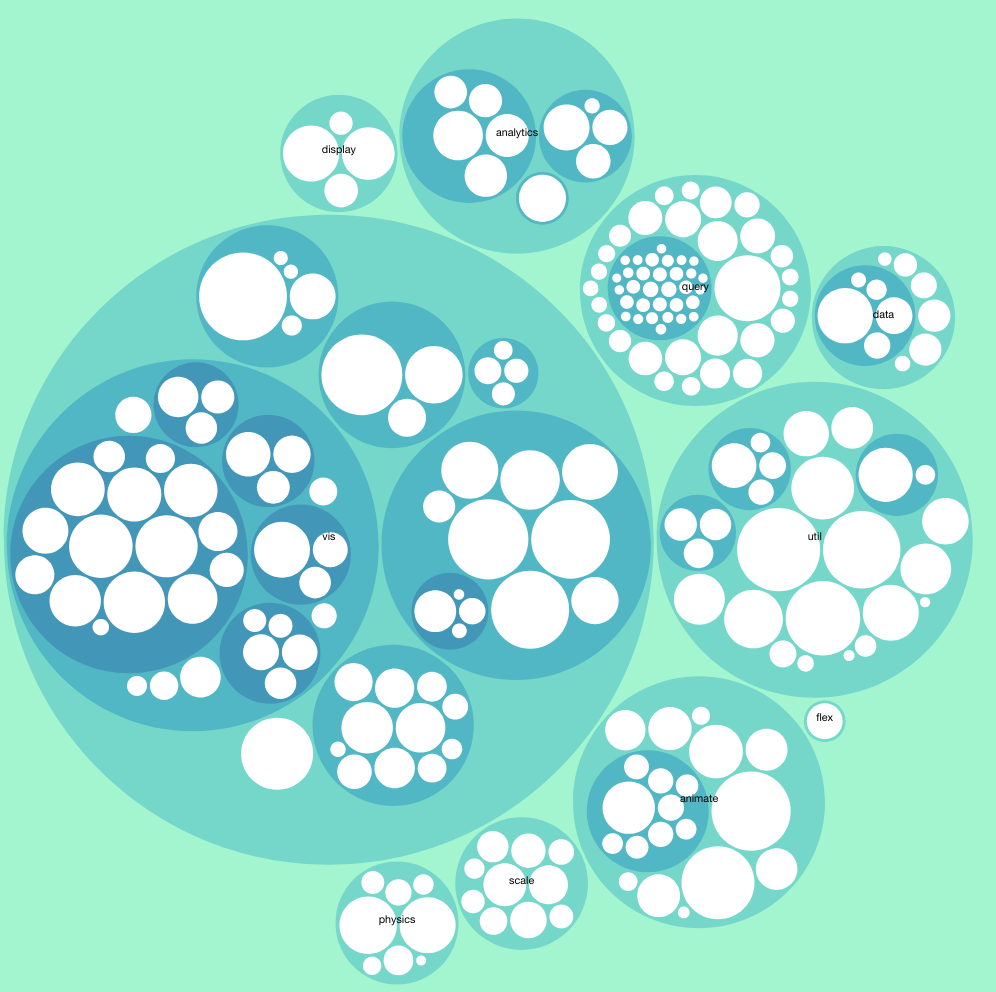
\includegraphics[width=0.8\textwidth]{imagenes/d3/ejemplo.png}
    \caption{Ejemplo de visualización generada con D3}
    \label{fig:d3-ejemplo}
\end{figure}

\section{D3}

D3 (Data-Driven Documents) es una librería de JavaScript para manipular documentas en función de datos. Esta librería permite manipular el DOM (Document Object Model) y aplicarle transformaciones según los datos. Permite usar las tecnologías estándar de la web para generar visualizaciones de buena calidad.

Es particularmente útil la capacidad de D3 de manipular elementos SVG (Scalable Vector Graphics) ---un lenguaje de markup para describir gráficos en dos dimensiones---. Esto permite generar animaciones en dos dimensiones de forma relativamente simple. Además esta técnica es bastante eficiente gracias a que los navegadores implementan motores muy eficientes para la renderización de elementos SVG.

Para lograr esto D3 permite enlazar datos con elementos del DOM y definir los atributos de estos elementos como función de los datos. Además, cuando cambian los datos se puede hacer una transición suave de los elementos correspondientes a su nueva posición según la función definida anteriormente. La figura~\ref{fig:d3-ejemplo} muestra un ejemplo de una visualización generada con D3 que representa un conjunto de datos como una agrupación de círculos.

\section{SUS}
\label{state-of-the-art:sus}

La escala SUS, o System Usability Scale utilizando su nombre completo, fue introducida en~\cite{brooke1996quick} por John Brooke como un método ``\textit{quick and dirty}'' (rápido y sucio) para evaluar usabilidad desarrollado en Digital Equipment Corporation. Desde entonces se ha vuelto un método estándar en la industria para medir la usabilidad en todo tipo de sistemas. En~\cite{evaluation-of-sus} analizan 10 años de datos de SUS y encuentran que esta escala es una herramienta altamente robusta y versátil para las evaluaciones de usabilidad.

SUS consiste en un formulario de 10 ítems que se le aplica a usuarios después de utilizar el sistema que se está evaluando. Cada ítem consiste de una afirmación para la cual el usuario debe marcar en una escala de 1 a 5 si está muy de acuerdo o muy en desacuerdo con la afirmación. Las afirmaciones están alternadas entre afirmaciones que reflejan positivamente y negativamente sobre la usabilidad, con el objetivo de obligar a los participantes a pensar sobre la respuesta de cada ítem. Las afirmaciones en la versión original son:
\begin{enumerate}
    \item I think that I would like to use this system frequently
    \item I found the system unnecessarily complex
    \item I thought the system was easy to use
    \item I think that I would need the support of a technical person to be able to use this system
    \item I found the various functions in this system were well integrated
    \item I thought there was too much inconsistency in this system
    \item I would imagine that most people would learn to use this system very quickly
    \item I found the system very cumbersome to use
    \item I felt very confident using the system
    \item I needed to learn a lot of things before I could get going with this system
\end{enumerate}

A partir de las respuestas del usuario se obtiene un puntaje entre 0 y 100. Para calcular el puntaje, cómo las preguntas están alternadas, primero se deben transformar los puntajes de forma que sean consistentes. Para esto, se transforma el puntaje de cada ítem a una escala entre 0 y 4, donde 0 es lo peor y 4 es lo mejor. Esto se logra restándole 1 a los ítems impares y restando de 5 los ítems pares. Después, sumando los puntajes transformados se obtiene un puntaje total entre 0 y 40, que se multiplica por 2.5 para obtener un puntaje entre 0 y 100.

En~\cite{quantifying-the-user-experience} reportan que utilizando datos de 446 estudios y más de 5000 respuestas individuales, encontraron que el promedio del puntaje fue 68 con una desviación estándar de 12.5. Por el mismo motivo recomiendan transformar el puntaje a un percentil para interpretar los resultados y presentan una tabla para transformar los puntajes a percentiles.

El cuestionario asociado a esta escala está en inglés, por lo que debe traducirse al español para aplicarlo a un grupo cuya lengua nativa es el español. 